\chapter{Hiding and Attacking Strategies}
\label{cha:STRATEGIES}

\section{Hiding}
Always hide self robot behind a obstacle and keep two robots and obstacle at a straight line, as shown in figure \ref{hiding_strategy}:

\begin{figure}[thb]
    \centering
    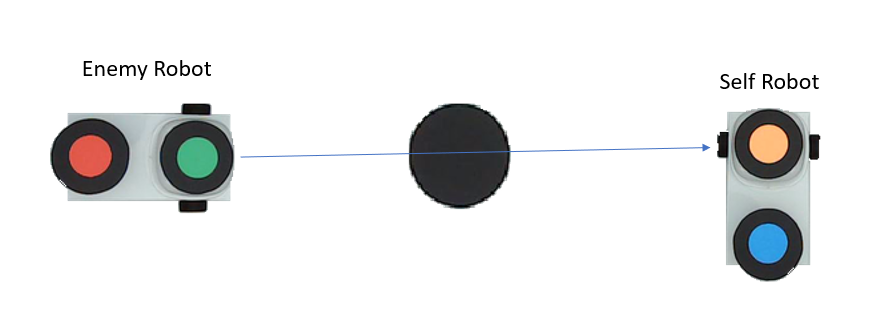
\includegraphics[width=1\textwidth]{images/hiding_strategy.png}
    \caption[hiding strategy]{an example of positions that satisfies the hiding strategy.}\label{hiding_strategy}
\end{figure}

 
In order to implement the strategies above, detail tactics will be introduced. As we can see in the figure  \ref{HidingModel}. Here we assume that there are three obstacles (1~3 obstacles in the environment randomly placed in the central part of the environment) in workspace. The red points are the centre of obstacles and robot,  $O$ point is the centre of opponent robot and $P$ point is the centre of my robot. In hiding model, my robot need to move to hidden point behind the obstacles quickly. But how to pick the specific hidden point is a difficult problem to be solved. There is a feasible solution to be introduced.

In the figure  \ref{HidingModel} . Three straight lines (auxiliary lines) pass through the center of the opponent robot and the center of the obstacle, they are line $OD$, line $OE$ and line $OF$. The vertical feet are point $A$, point $B$ and point $C$, when make vertical lines from point $P$ to these three lines— line $OD$, line $OE$, line $OF$. My robot will regard $C$ point as the best hidden point. Compared with other hidden points ($A$ position and $B$ position) $C$ is the nearest point where to the current my robot position. According to the position of obstacles and robots (my robot and opponent robot), hidden model will update the dynamic hidden point to avoid the hit and attack from opponent robot.

\begin{figure}[thb]
    \centering
    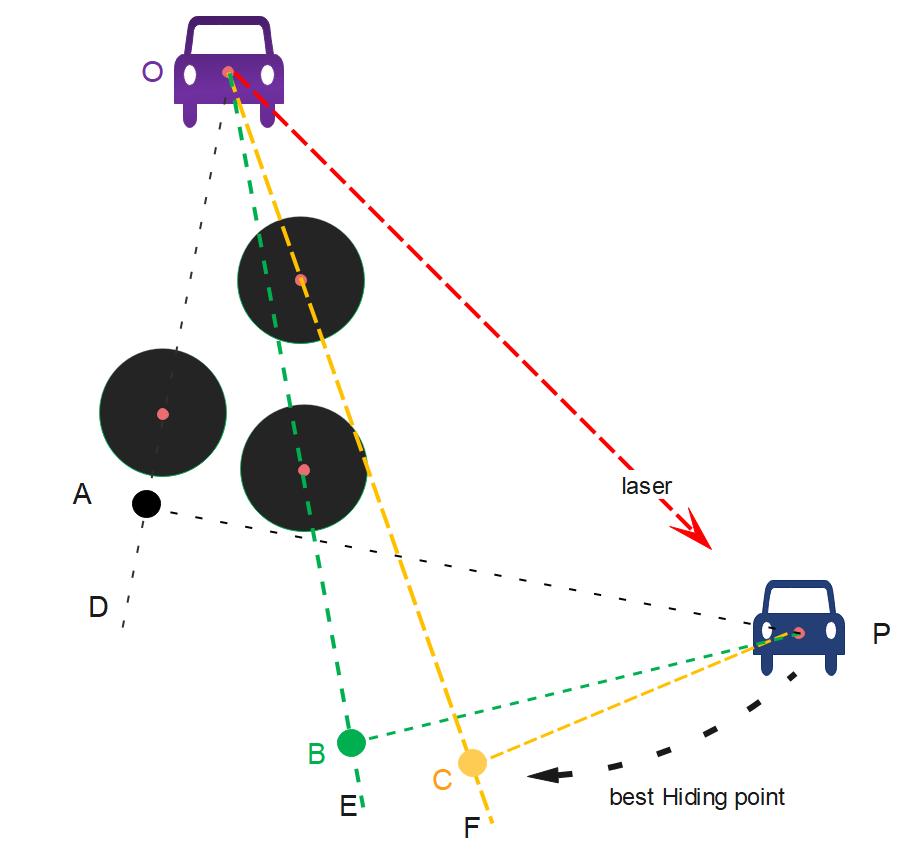
\includegraphics[width=1\textwidth]{images/PathPlaningHidingModel.png}
    \caption[hiding strategy]{Principle of finding the optimal hidden point}\label{HidingModel}
\end{figure}



\section{Attacking}
Since there is only one chance to fire the laser, it should fire until there is no obstacle between two robots. In order to do so, attacking robot should chase another robot. 

Method 1:
Move the robot to the position of another robot as soon as possible.

Method 2:
Searching the nearest point that is at the straight line with another robot without an obstacle as shown in figure \ref{attacking_method2}:

\begin{figure}[thb]
    \centering
    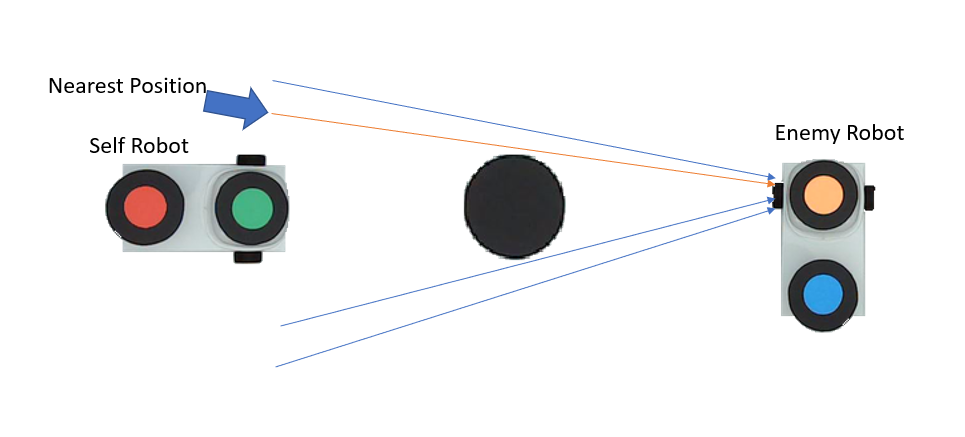
\includegraphics[width=1\textwidth]{images/attacking_method2.png}
    \caption[attacking method]{an example of positions that satisfies the attacking strategy.}\label{attacking_method2}
\end{figure}
